\documentclass[compress]{beamer}
\usepackage[utf8]{inputenc}
\usepackage[francais]{babel}
\usepackage[T1]{fontenc}
\usepackage{amssymb}
\usepackage{amsmath}
\usepackage{amsfonts}
\usepackage{hyperref}
\usepackage[]{algorithm2e}
\usepackage{amssymb}
\usepackage{verbatim}
\usepackage{listings}
\usepackage{color}
\usepackage{graphicx}
\usepackage{subfig}

\usepackage{wrapfig} % in preamble
\usetheme[navigation]{UMONS}

\author{Benjamin André, Alexis Lecocq}
\title{Statistiques multidimensionnelles}
\subtitle[\ldots]{Réseaux de neurones (NN)}

\setbeamercovered{transparent} 
\setbeamertemplate{navigation symbols}{} 
\institute{UMONS\\Faculté des Sciences\\BA 3 Sciences Informatiques\\[2ex]
  
\includegraphics[height=4ex]{UMONS}\hspace{2em}%
  \raisebox{-1ex}{
\includegraphics[height=6ex]{UMONS_FS}}}
\date{Juin 2017} 
\definecolor{darkgreen}{rgb}{0.0, 0.2, 0.13}
\subject{Statistiques multidimensionnelles} 
\lstset{ %
  language=R,                     % the language of the code
  basicstyle=\footnotesize,       % the size of the fonts that are used for the code
  numbers=left,                   % where to put the line-numbers
  numberstyle=\tiny\color{gray},  % the style that is used for the line-numbers
  stepnumber=1,                   % the step between two line-numbers. If it's 1, each line
                                  % will be numbered
  numbersep=5pt,                  % how far the line-numbers are from the code
  backgroundcolor=\color{white},  % choose the background color. You must add \usepackage{color}
  showspaces=false,               % show spaces adding particular underscores
  showstringspaces=false,         % underline spaces within strings
  showtabs=false,                 % show tabs within strings adding particular underscores
  frame=single,                   % adds a frame around the code
  rulecolor=\color{black},        % if not set, the frame-color may be changed on line-breaks within not-black text (e.g. commens (green here))
  tabsize=2,                      % sets default tabsize to 2 spaces
  captionpos=b,                   % sets the caption-position to bottom
  breaklines=true,                % sets automatic line breaking
  breakatwhitespace=false,        % sets if automatic breaks should only happen at whitespace
  title=\lstname,                 % show the filename of files included with \lstinputlisting;
                                  % also try caption instead of title
  keywordstyle=\color{blue},      % keyword style
  commentstyle=\color{darkgreen},   % comment style
  stringstyle=\color{violet},      % string literal style
  escapeinside={\%*}{*)},         % if you want to add a comment within your code
  morekeywords={*,...}            % if you want to add more keywords to the set
} 




\begin{document}

	\begin{frame}
		\titlepage
	\end{frame}

	\begin{frame}
		\tableofcontents
	\end{frame}

	\section{Description des NN}
		\subsection{Machine Learning}
			\begin{frame}
				\frametitle{Machine Learning}
				\begin{wrapfigure}{l}{0.5\linewidth}
					\vspace{-2em}
					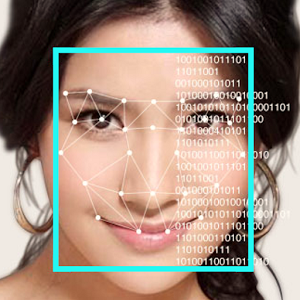
\includegraphics[width=\linewidth]{img/faced}
				\end{wrapfigure}
				
				Certains problèmes comme la reconnaissance faciale comportent trop de variables et des relations trop compliquées entre celles-ci pour être décrite efficacement de façon algorithmique.
				
				On préférera le machine learning qui proposera une solution approchée grâce à l'apprentissage automatique.
			\end{frame}
			
			\begin{frame}
				\frametitle{Machine Learning}
				\begin{alertblock}{Utilisation}
					Comme expliqué précédemment, il s'agit d'une solution approchée. Dans le cas ou il existe un algorithme efficace il sera préférable de l'utiliser.
				\end{alertblock}
				
				\begin{block}{Exemples}
					\begin{itemize}
						\item AlphaGo
						\item DeepBlue
						\item Voitures autonomes
						\item Filtre à spam
						\item Reconnaissance d'image
						\item Traduction
						\item Prévision de la bourse
					\end{itemize}
				\end{block}
			\end{frame}
		\subsection{Neural Networks (NN)}
			\begin{frame}
				\frametitle{Neural Networks}		
				\hspace{3em}%
				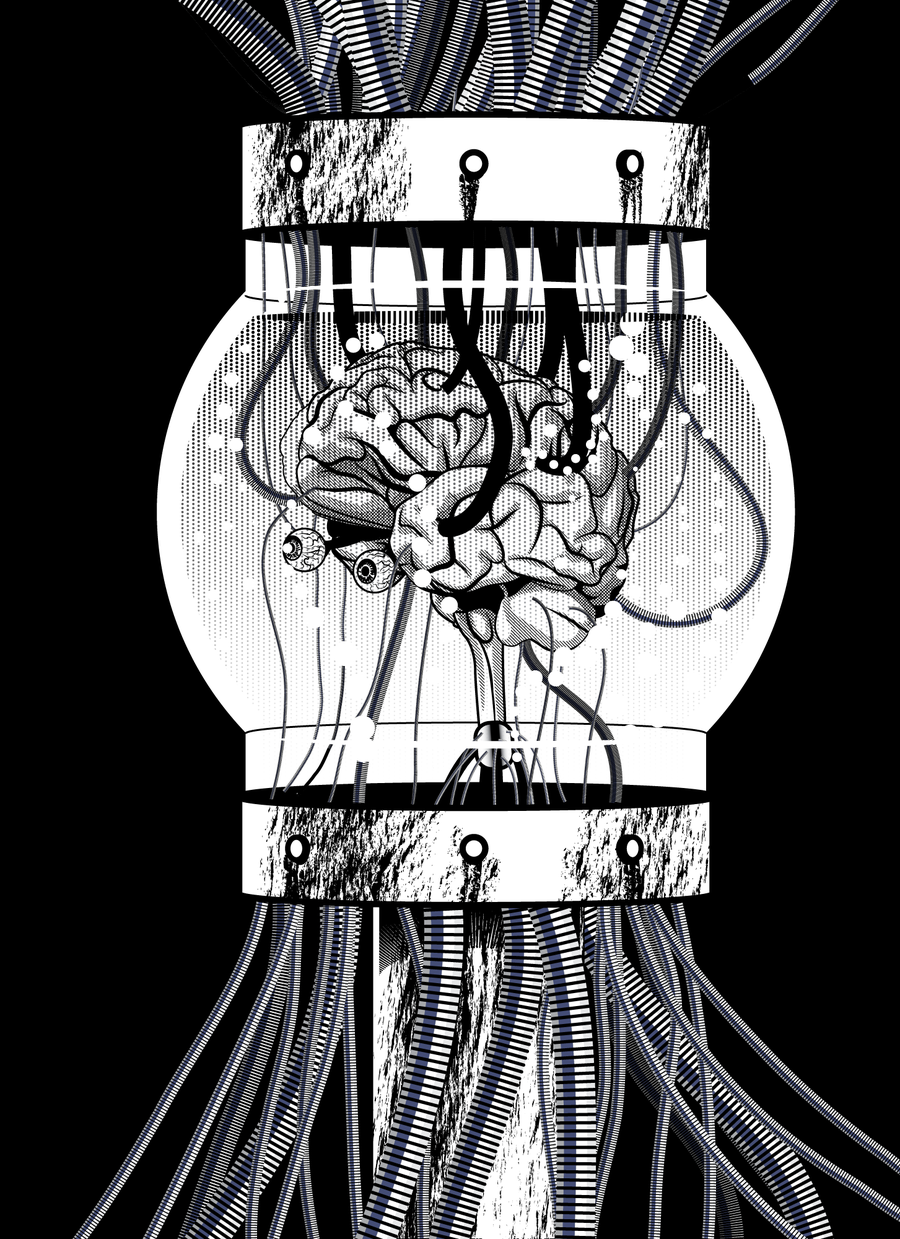
\includegraphics[height=100px]{img/brain}\hspace{2em}%
				\raisebox{-1ex}{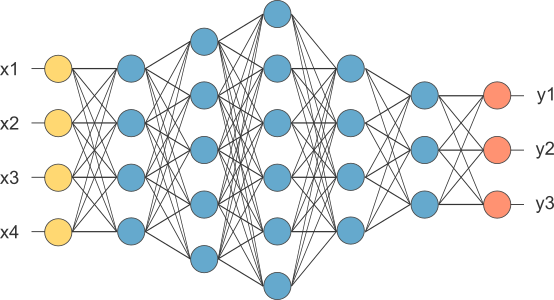
\includegraphics[height=100px]{img/deep_neural_network}}
				
				%Et ici on fait la blague qu'on pourrait penser au cerveau connecté et que ça fait peur, mais qu'en réalité... ça fait encore plus peur !
			\end{frame}


			\begin{frame}
				\frametitle{Neural Networks}
				\begin{block}{Types de réseaux de neurones}
					\begin{itemize}
						\item Deep Neural Network (DNN) : Réseau avec un grand nombre de couches.
						\item Convolutional Neural Network (CNN) : Inspiré du fonctionnement de la vue, les couches de neurones ici sont à plus d'une dimension.
						\item Recurrent Neural Network (RNN) : Réseau où la sortie est réintroduite dans le réseau pour les tests suivants : effet mémoire. 
					\end{itemize}
				\end{block}
				
				=> Nous utiliserons une version généraliste de la technique, fonctionnant comme un DNN avec peu de couches.
			\end{frame}
	
			
			\begin{frame}
				\frametitle{Fonctionnement global}
					Comment trouver $f(x_1, x_2, ..., x_n)$ ?
				
					On l'écrit sous la forme $f(x_1, x_2, ..., x_n) = a(w_1 * z_1, w_2 * z_2, ..., w_n * z_n)$
					
					Où $z_i$ pourrait lui-même être le résultat d'une fonction mathématique.
					
					En composant les fonctions (avec un certain poids $\vec{w}$) jusqu'à des fonctions simples sur $\vec{x}$, on crée un réseau de neurones (fonctions).
				
					A force d'exemples, on ajuste les \emph{poids} (axones) $w_i$ afin d'approximer $f$.
			\end{frame}


		\subsection{Formulation générale}
			\begin{frame}
				\frametitle{Structure des couches}
				3 types de couches :
				\begin{itemize}
					\item L'entrée : Couche correspondant aux variables à évaluer
					\item Les couches "cachée" : Couches correspondant au comportement interne du réseau, le nombre de couches dépend du problème, et il n'y a pas de règles prédisant le nombre de couches nécessaires. De nombreuses opérations mathématiques se font ici.
					\item La sortie : Couche retournant un nombre correspondant soit à une classe, soit à la valeur d'évaluation des paramètres d'entrées
				\end{itemize}
				
				Aucun neurone (décrits plus tard) n'est dans plusieurs couches. Ceux-ci sont interconnectés avec tous les neurones de la couche précédente et tous ceux de la suivante, et rien d'autre (parfois avec un poids 0 cependant).
				
			\end{frame}


			\begin{frame}
				\frametitle{Couche cachée}
				\hspace{6em}%
				\vspace{6em}
				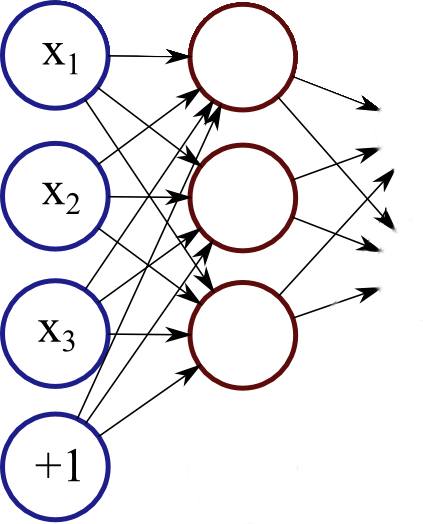
\includegraphics[height=120px]{img/hidden_layer}\hspace{2em}%
				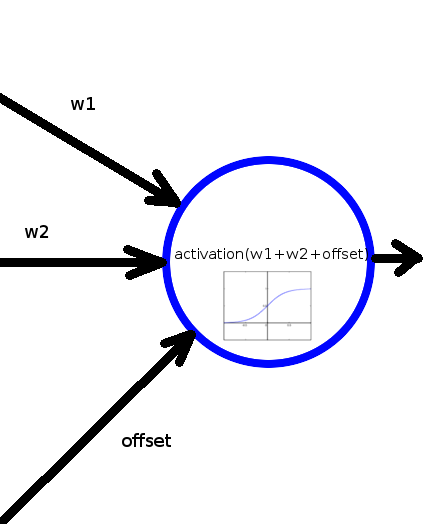
\includegraphics[height=120px]{img/neurone}
				\vspace{-4em}				
			\end{frame}
			
			\begin{frame}
				\frametitle{Fonction d'activation}
				
				Chaque neurone effectue la somme pondérée par $w$ de tous les résultats de la couche précédente.\\
				Par exemple : $(0.2*w1 + 1.4*w2 - 2.1)$.\\
				Pour à cette somme, nous appliquons une fonction dite "d'activation".
				
				La fonction d'activation appliquée sur la transformation linéaire la plus répandue est la sigmoïde: 
				$$  activation(x) = \frac{1}{1 + e^{-x}} \in \left[0, 1\right] $$				
			\end{frame}

			\begin{frame}
				\frametitle{Fonction d'activation}
				
				Cette fonction a plusieurs propriété intéressantes :
				\begin{itemize}
					\item $activation(x) \in [0, 1]$, utile pour borner le résultat et éviter une explosion des valeurs dans le réseau
					\item Fonction continue sur $\Re$
					\item Elle est dérivable en $activation(x) * (1 - activation(x))$, ce qui est utilisé dans le calcul de l'erreur
				\end{itemize}
			\end{frame}

			\begin{frame}
				\frametitle{Représentation}
				\vspace{-2em}
				\centerline{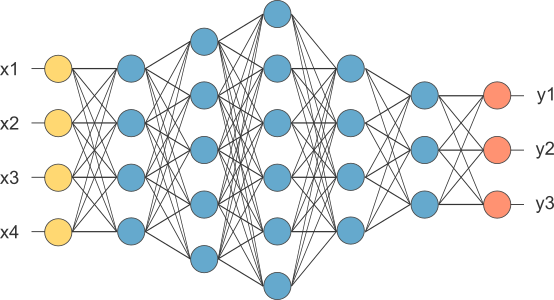
\includegraphics[width=0.3\linewidth]{img/deep_neural_network}}
				\vspace{-1em}
				\[
					x = 
					\begin{pmatrix}
					x_1\\x_2\\x_3\\x_4
					\end{pmatrix}
					,
					w_1 = \begin{pmatrix}
					w_{{x_1}{h_1}} & w_{{x_1}{h_2}} & w_{{x_1}{h_3}} & w_{{x_1}{h_4}} \\
					w_{{x_2}{h_1}} & w_{{x_2}{h_2}} & w_{{x_2}{h_3}} & w_{{x_2}{h_4}} \\
					w_{{x_3}{h_1}} & w_{{x_3}{h_2}} & w_{{x_3}{h_3}} & w_{{x_3}{h_4}} \\
					w_{{x_4}{h_1}} & w_{{x_4}{h_2}} & w_{{x_4}{h_3}} & w_{{x_4}{h_4}}
					\end{pmatrix}				
					,
					w_2 \in \Re^{4x5}
					, ... ,
					y = 
					\begin{pmatrix}
					y_1\\y_2\\y_3
					\end{pmatrix}
					.
				\]			
								
				Sans oublier les offset pour chaque couche, stockés séparément. On représente donc notre problème sous la forme matricielle.
								
				\end{frame}

			\subsection{Backpropagation}
			\begin{frame}
				\frametitle{Backpropagation}
				\begin{alertblock}{C'est fini ?}
					On a un réseau de neurones, c'est bien beau, mais comment définir les poids ?
				\end{alertblock}
				
				Plusieurs stratégies pour l'initialisation dont l'aléatoire.
				Ensuite on nourri le réseau d'exemples. On mesure le taux d'erreur entre l'approximation et les données de résultat. A chaque fois, un algorithme appelé \emph{backpropagation} est appliqué pour ajuster les poids \emph{en détectant lequel est le plus responsable de l'erreur}.
			\end{frame}
			
			\begin{frame}
				\frametitle{Backpropagation}
				Sans entrer trop dans les détails, ce que fait l'algorithme :
		
		\begin{tiny}
				\begin{algorithm}[H]
					\SetKwData{Left}{left}\SetKwData{This}{this}\SetKwData{Up}{up}
					\SetKwFunction{Union}{Union}\SetKwFunction{FindCompress}{FindCompress}
					\SetKwInput{Entree}{Entrées}
					\SetKwInput{Effet}{Effets}
					\SetKwInput{Sortie}{Sorties}
					\SetKw{Retour}{retourner}
					\SetKwFor{Pour}{pour}{faire}{finpour}
					\SetKwFor{Tq}{tant que}{faire}{fintq}
					\SetKwFor{PourCh}{pour chaque}{faire}{fait}
					\SetKwFor{PourTous}{pour tout}{faire}{fait}
					\SetKwRepeat{Repeter}{répéter}{jusqu'à}
					\SetKwIF{Si}{SinonSi}{Sinon}{si}{alors}{sinon si}{sinon}{{fin si}}
					\SetKwSwitch{Match}{Case}{Other}{match}{ : }{cas}{autre cas}{{fin cas}}{{fin match}}
					\Entree{Un jeu de données}
					\Sortie{Les poids}
					$w$ $\leftarrow$ valeurs aléatoires entre -1 et 1\\
					\Repeter{nombre d'itération maximum atteint ou l'erreur globale est passée sous un seuil fixé}{
						\PourCh{$exemple$ du training set}{
							\PourCh{$couche$ dans le 	réseau}{
								\PourCh{$noeud$ dans la $couche$}{
									$sum$ $\leftarrow$ la somme des entrées\\
									$sum$ $\leftarrow$ $sum + offset$\\
									$noeud_{sortie}$ $\leftarrow$ $activation(sum)$
								}
							}
							
							\PourCh{$noeud$ dans la couche de sortie}{
								$node_{error} \leftarrow \Delta(attendu, calculé)$						
							}
							
							\PourCh{couche cachée dans le réseau}{
								\PourCh{$noeud$ dans la couche}{
									Calculer $node_{error}$\\
									Mettre à jour le poids du n\oe ud dans le réseau.							
								}
							}
							
							Calculer l'erreur globale
						}
					}
					\Retour $arbre$
					\BlankLine
				\end{algorithm}
		\end{tiny}
				
			
			\end{frame}
			
			\begin{frame}
				\frametitle{Backpropagation}
				Pour faire simple :
				\begin{itemize}
					\item On initialise les poids aléatoirement
					\item On présente un exemple et évalue l'erreur
					\item On fait remonter l'erreur en fonction des poids
					\item On ajuste les poids en fonction de l'erreur et continue à faire remonter l'erreur
					\item On donne un autre exemple, et s'arrête après un certain temps ou si le NN est efficace
				\end{itemize}
			\end{frame}

			\begin{frame}
				\frametitle{Backpropagation}
				\vspace{-2em}
				\centerline{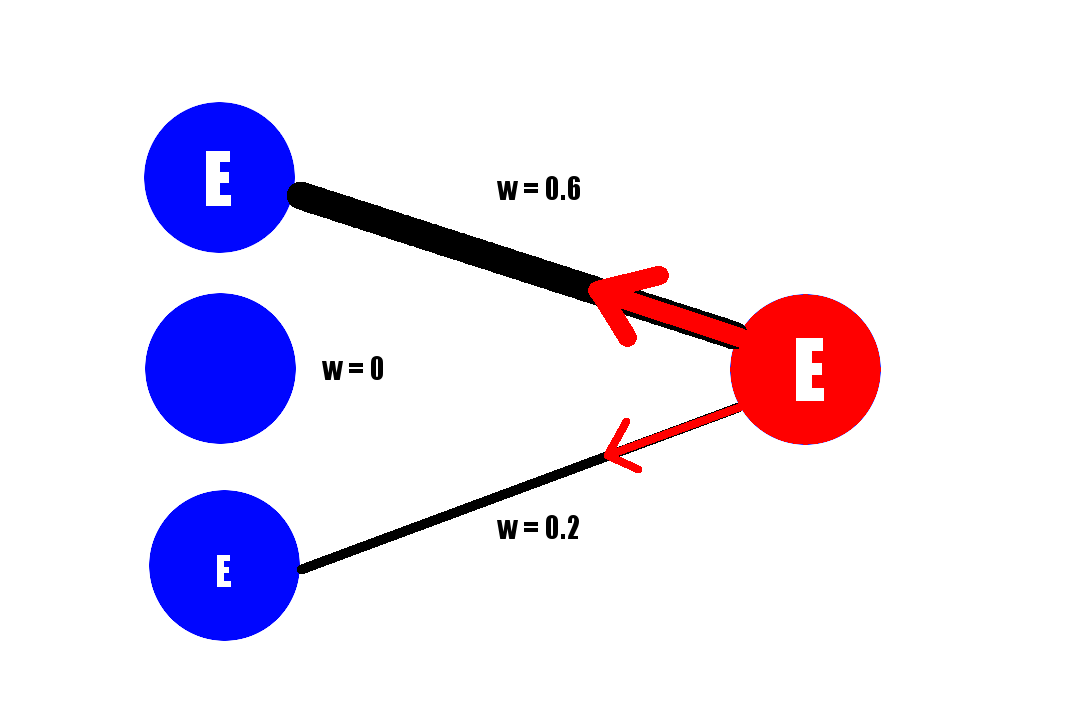
\includegraphics[width=0.8\linewidth]{img/bprop}}
			\end{frame}

			
	
	
	\section{Exemple en R}
		\subsection{Choix de librairie}
		\begin{frame}
			\frametitle{Choix de librairie}
			La librairie choisie est \textbf{neuralnet}. C'est une librairie de très haut niveau, mise à jour régulièrement, documentée, et avec une certaine communauté (qui a d'ailleurs écrit un tutoriel).
		\end{frame}
		
		\subsection{Données utilisées et objectif}
		\begin{frame}
			\frametitle{Données utilisées et objectif}
			\begin{wrapfigure}{l}{0.5\linewidth}
				\vspace{-2em}
				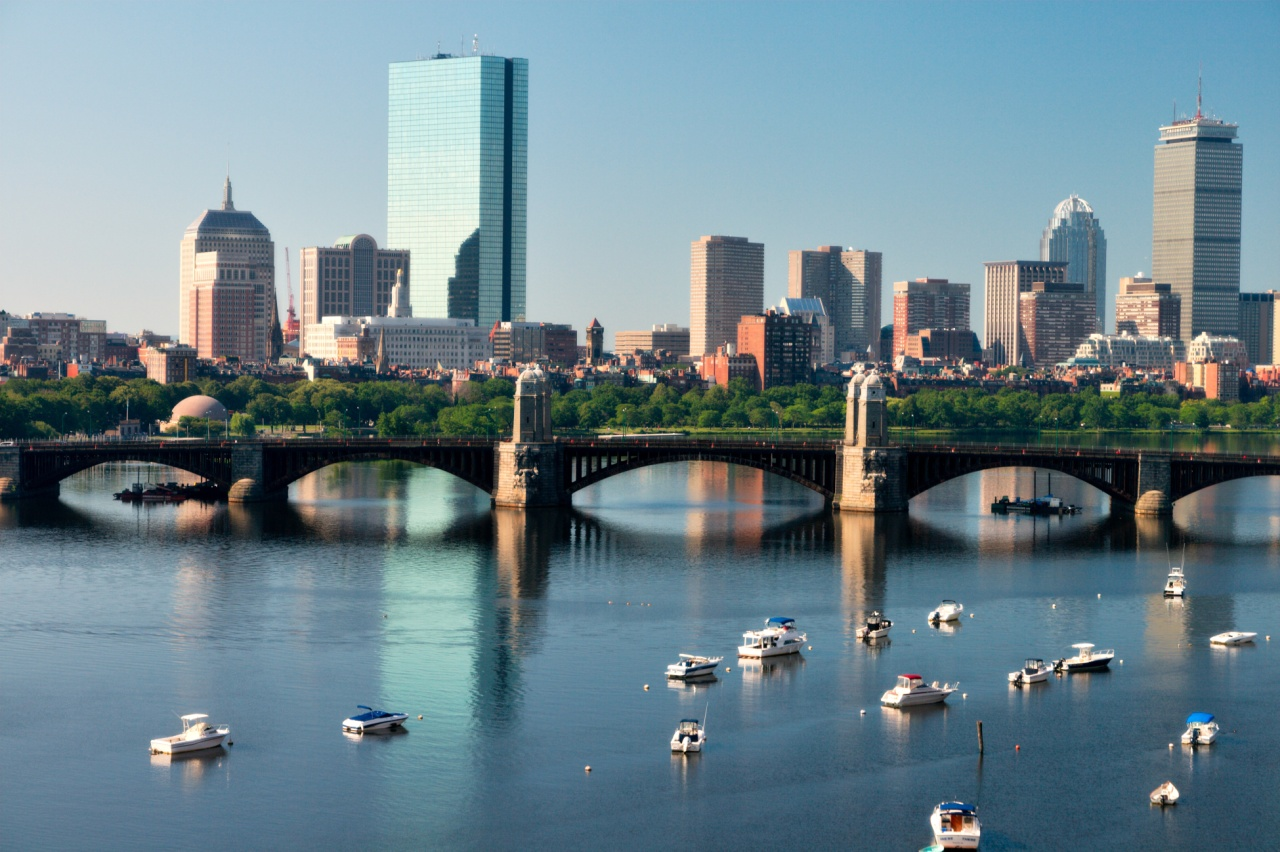
\includegraphics[width=\linewidth]{img/boston}
			\end{wrapfigure}
			On utilisera les données "Boston" fournies de base par RStudio. Celles-ci mettent en relation 13 variables sur une propriété et sa valeur.
			\\
			Notre but sera de prédire la valeur d'un bâtiment en fonction des 13 variables.
			
		\end{frame}
		
			
		\subsection{Traitement des données}
%		\subsection{Vérification}
%		\subsection{Séparation des données}
%		\subsection{Normalisation de la matrice des variables}
		\subsection{Entraînement}
		%\subsection{Test sur les données restantes}
		\subsection{Comparaison du résultat du NN avec la réalité}
		\subsection{Fiabilité du réseau}
		%Test sur 10 exemples (melange des donnes)
		%Pour generer une probabilite sur l'erreur de notre reseau
		%Boite a moustache

\section*{Sources}
\begin{frame}
\frametitle{Sources}
	\url{https://www.r-bloggers.com/fitting-a-neural-network-in-r-neuralnet-package/}\\
	\url{http://www.parallelr.com/r-deep-neural-network-from-scratch/}\\
	\url{https://www.youtube.com/watch?v=BR9h47Jtqyw}\\
	\url{http://doctor-morbius.deviantart.com/}\\
	\url{https://datascienceplus.com/fitting-neural-network-in-r/}%d'ou on tient le code !
	\url{https://play.google.com/store/apps/details?id=com.seakleng.facedetection&hl=fr}
\end{frame}

\end{document}